\documentclass[titlepage=firstiscover,11pt,fleqn,headheight=14pt,footheight=40.8pt]{scrreprt}

%template includes
\usepackage{amsmath}
\usepackage{cite}
\usepackage{multirow}
\usepackage{pslatex}
\usepackage{xspace}
\usepackage[euler]{textgreek} % allows use of greek in text without mathmode
\renewcommand{\bibname}{References} % changes bibliography title to references
\usepackage{subcaption}
\usepackage{booktabs}
\usepackage{longtable}
\usepackage{pgfplots}
\pgfplotsset{compat=1.10}
\usepackage{pgfplotstable}
\usepackage[font=small]{caption}
\usepackage[capitalise]{cleveref} % allows use of sorting of multiple references
\usepackage{authblk} % author afiliations
\usepackage{wasysym} % use circles
\usepackage{scrlayer-scrpage} % header and footer

%original includes
%\usepackage[letterpaper]{geometry} 
%\widowpenalty=1000
%\clubpenalty=1000
%\biboptions{numbers,sort&compress}
%\usepackage[utf8]{inputenc} % set input encoding (not needed with XeLaTeX)
%\usepackage[small,bf]{caption}
%\usepackage[T1]{fontenc}
%\usepackage{graphics,array}
%\usepackage{kpfonts}
%\usepackage{avant}
%\usepackage{mathpazo}
%\usepackage{mathpazo}
%\usepackage{color}
%\usepackage[usenames,dvipsnames]{xcolor}
%\usepackage{graphicx} % support the \includegraphics command and options
%\usepackage{booktabs} % for much better looking tables
%\usepackage{array} % for better arrays (eg matrices) in maths
%\usepackage{subfig}
%\renewcommand{\baselinestretch}{1.2}
%\renewcommand{\familydefault}{\sfdefault}

%\usepackage[bottom]{footmisc} %footnote at botton of page
%\usepackage{amsmath}
%\usepackage{multicol}
%\pagenumbering{gobble}
%\pagenumbering{arabic}
%\makeatletter
%\def\ps@pprintTitle{%
%  \let\@oddhead\@empty
%  \let\@evenhead\@empty
%  \let\@oddfoot\@empty
%  \let\@evenfoot\@oddfoot
%}
%\makeatother

%\biboptions{}

\graphicspath{
{figures/}
}

\begin{document}

\setkomafont{author}\large
\setkomafont{date}\large

%\titlehead{\centering \includegraphics[scale=.8]{figures/logo.png}}
%\subject{Small heading (optional)}
\title{}
%\subtitle{asdf}

\date{Predicting thermodynamic and thermophysical properties of molten chloride salts from ab-initio molecular dynamics simulations}

\maketitle

\tableofcontents

\chapter{Introduction}

\chapter{Case study: Ab initio molecular dynamics simulations of select thermophysical and thermodynamic properties of NaCl, UCl$_3$ and NaCl-UCl$_3$ molten salts}
\label{sec:NaCl}

\section{Review of existing experimental and modeling studies on NaCl, UCl$_3$ and NaCl-UCl$_3$}
Experimental characterization of UCl$_3$ densities have been reported by Janz et al.\cite{Janz1988} and Desyatnik et al.~\cite{Desyatnik}. The density correlations derived from these two experimental data sets deviate significantly from each other. Desyatnik et al.~\cite{Desyatnik} also investigated the density of NaCl-UCl$_3$ mixtures. They identified a negative deviation from an ideal solution across most of the composition range, with the high-temperature UCl$_3$ region deviating slightly from this trend. 
Maatsura et al.~\cite{Matsuura} measured the mixing energies of NaCl-UCl$_3$ at 1173 K, which highlighted a negative deviation from ideal solution behavior, which implies an exothermic reaction, with a shallow minimum of $-0.07$ to $-0.08$ eV per formula unit close to the eutectic composition ($x_{UCl_3}\approx 0.35$), but perhaps slightly shifted towards the 50-50 composition. There are two Calphad assessments of the NaCl-UCl$_3$ system~\cite{BENES2008, YIN2020}. The magnitude and shape of the NaCl-UCl$_3$ mixing energies are noticeably different between the two assessments~\cite{YIN2020}. The assessment by Benes et al.~\cite{BENES2008} arrived at a form with a minimum close to the eutectic composition ($x_{UCl_3}\approx 0.35$), while Yin et al.~\cite{YIN2020} used the experimental data due to Matsuura et al.~\cite{Matsuura} as input, which resulted in a more negative mixing energy that is shifted slightly closer to the 50-50 composition. The magnitude of the mixing energy is off by about 50\% between the two assessments. 

The sparse and sometimes contradictory experimental data on molten salts in general and the NaCl-UCl$_3$ system in particular provide justification for pursuing modeling and simulations as a complementary approach to gain improved understanding. This opportunity is already acknowledged  in the literature. Molecular dynamics simulations based on both classical potentials and AIMD simulations have been used to study chloride salts involving actinides~\cite{Li,Li2020,Nam2015,SONG}. Li et al.~\cite{Li} used AIMD simulations to study the local structure of UCl$_3$, UCl$_4$ and mixtures of UCl$_3$, UCl$_4$ and NaCl at 1173 K. This study showed good agreement with experiments for the radial distribution function of the first coordination shell and identified network formation of UCl$_3$ units in mixed NaCl-UCl$_3$ salts~\cite{Li}. %radial distribution function. 
In order to study temperature dependent thermo-physical properties, a semi-empirical potential was developed~\cite{Li2020}. This potential successfully predicted density, thermal conductivity and viscosity, though validation is challenged by the lack of experimental data. Nam et al.~\cite{Nam2015} studied the solution thermodynamics of dilute concentrations of UCl$_3$ in a base salt and investigated the properties of base salts for different Van der Waals interaction models. Song et al.~\cite{SONG} performed AIMD simulations of densities and transport properties in a LiCl-KCl eutectic salt with a small concentration of UCl$_3$. 

In the present study, AIMD simulations relying on different models for the Van der Waals interactions were used to predict temperature dependent thermophysical (density) and thermochemical (mixing energy and heat capacity) properties of NaCl, UCl$_3$ and NaCl-UCl$_3$. The standard PBE exchange-correlation potentials typically used were extended to include a Hubbard $U$ model for the actinide 5f electrons. The purpose of the study was first to determine with what accuracy fundamental properties can be predicted with AIMD simulations for actinide containing salts, second to populate some of the data gaps that exist in the literature and third to provide understanding of the link between coordination chemistry and properties. 

The next sections are organized as follows. The methodology is described in Sec. \ref{sec:method}, followed by results and discussion in \ref{sec:results}. First the benchmark for NaCl is presented, next the UCl$_3$ results are reviewed, which is followed by NaCl-UCl$_3$ mixtures. The connection of our results to local chemistry and pair distribution functions are discussed in Sec. \ref{sec:discussion}. % and, finally, our conclusions are presented in Sec. \ref{sec:conclusions}. 

\section{Methodology}
\label{sec:method}
%\subsection{DFT methodology}
The AIMD simulations were performed with the VASP code~\cite{Kresse1996}. The simulations used a range of supercell sizes with the largest consisting of 216 (NaCl), 216 (UCl$_3$) and 134-184 (NaCl-UCl$_3$ mixtures) atoms. The smallest cells for the same systems contain 64, 64 and 60-72 atoms, respectively. %Further details will be provided in Sec. \ref{sec:results}. 
For NaCl and UCl$_3$ these were created by expansion of the crystalline unit cells followed by melting of the lattice by performing high temperature MD simulations. % or by application of the PACKMOL package followed by high temperature annealing of the structures. 
%by expansions of the crystalline unit cells followed by melting of the lattice by performing high temperature molecular dynamics runs, to be described later in this section, or by XXX. 
The mixed supercells were created by replacing Na ions with U ions or vice versa, in some cases additional molecular units were added to ensure that an suitable number of atoms were maintained in the supercells. % similar procedures. 
%by expansion of the crystalline unit cells followed by melting of the lattice either by performing high temperature molecular dynamics simulations, or direct high temperature AIMD simulations.
The differently sized supercells were investigated in order to understand and optimize the compromise between computational efficiency, enabling sampling in the time domain, and accuracy with respect to long range interactions. The radial distribution function (RDF) was used as the most basic measure of the adequacy of the supercell size, with convergence with respect to the targeted thermophysical and thermodynamic properties following suite. 
All the supercells investigated properly capture the expected radial distribution function in the liquid state. %The radial distribution function was confirmed to reach a value close to one for  radii larger than 8-10 \AA. The convergence is slowest for network forming ions such as uranium~\cite{}. 
This behavior is exemplified in Figures \ref{fig:radial}a) and \ref{fig:radial}b) for two UCl$_3$ and NaCl supercells of different size, respectively. %, which also compares our results to the existing literature~\cite{}. 
The smaller cells predict essentially identical radial distribution functions to the larger cells, but come with improved computational efficiency. % compromise some accuracy in the radial distribution function for computationally efficiency. %, as will be quantified in Sec.~\ref{sec:results}. 
Although the larger cells may still be more accurate for, e.g., mixed salts exhibiting more complex radial distribution functions, the situation in mixed salts is further complicated by the need to sample sufficient configurations to resolve the preferred short and intermediate range distribution of ionic species in network forming salts such as UCl$_3$~\cite{Li}. This requires fairly long simulation times. %, especially for mixed salts in the constant pressure ensemble. 
Proper sampling is easier to achieve in smaller supercells given the computational cost of AIMD simulations, even though the radial distribution itself as well as other properties may be better described in a larger supercell. For this reason, our production runs tend to use supercells of intermediate size.  Based on the verification against large supercells for the radial distribution function above and further examples in Sec. \ref{sec:results}, the results in the present study are considered sufficiently converged with respect to supercell size.

All simulations used the $\Gamma$ point for integration in reciprocal space. The accurate simulation setting was utilized in VASP, but the plane wave cut-off energy was increased above the standard setting to 400 eV. Gaussian smearing with a smearing parameter of 0.05 eV was used for the partial occupancies of the wave functions. The convergence criteria for the electronic minimization was at least10$^{-3}$ eV for NaCl and $5\times10^{-3}$ eV for salts containing uranium. 

\begin{figure*}[htb]
\centering
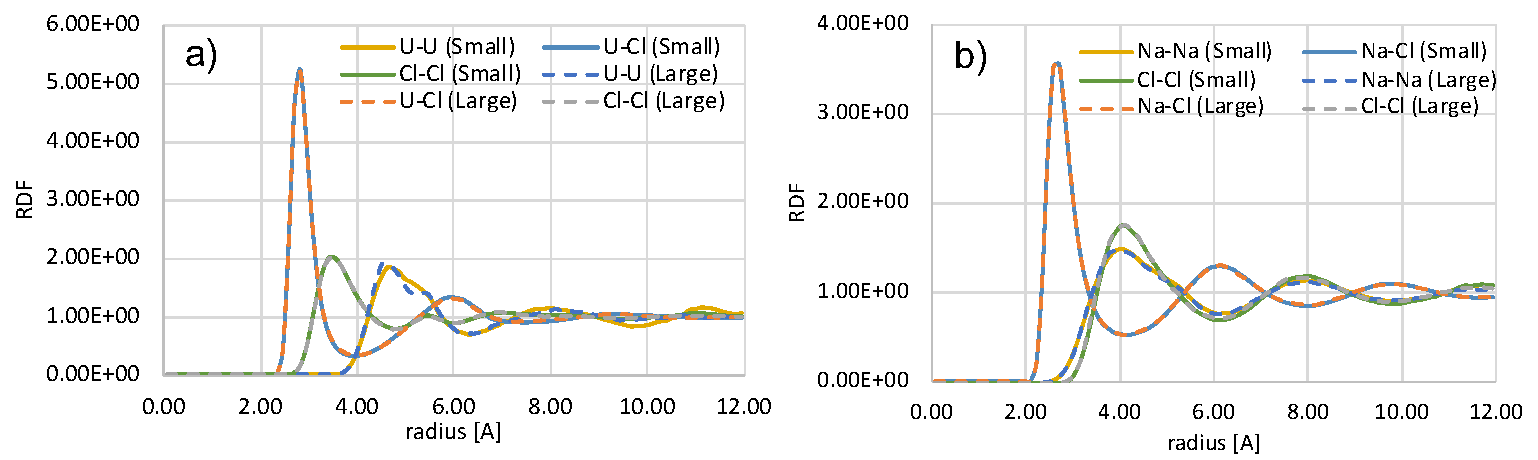
\includegraphics[width=0.95\textwidth]{FIG1_0.pdf}
\caption{The predicted radial distribution function in a) UCl$_3$ and b) NaCl obtained by supercells containing 64 (small) and 216 (large) atoms at 1250 K.} 
\label{fig:radial}
\end{figure*}

The Projector Augmented Wave (PAW) method was used to describe the core electrons~\cite{PAW1,PAW2}. For each element, the PAW potentials supplied with VASP for the PBE exchange-correlation potential were utilized. For Na, the version that only includes the s electron(s) in the valence shell was used. % for some of the simulations.%, while others use the version that also includes the semi-core p electrons. %The difference between the two potentials will be discussed in Sec. \ref{sec:results}. 
%Calculation of, for example, mixing energies in UCl$_3$-NaCl, can only be performed using a self-consistent data set (the same PAW potential), a rule which is carefully enforced in the present study. 
The PAW potential for Cl also included p electrons and for U it included the outer s, p and f electrons in the valance shell. %For some of the Van der Waals models, an alternate exchange-correlation potentials was utilized (rPW86~\cite{}). 
Calculations for U ions were performed with a Hubbard $U$ term, in order to capture the impact of accounting for strong electron correlation effects. 
%than PBE, such as XX, were used.
%For the uranium 5f electrons, an additional Hubbard $U$  term was introduced in order to capture the effect of strong correlations. 
%Calculations were also performed with the standard exchange-correlation potential (no Hubbard $U$ model). 
The Lichtenstein approach~\cite{PhysRevB.52.R5467} was used for the Hubbard $U$ methodology. An approximate $U$ value range of 3.0-4.5 eV was determined by using scoping constrained DFT linear-response method for crystalline UCl$_3$~\cite{PhysRevB.71.035105}. 
The $J$ value was set to 0.51 eV. These values are similar to those proposed for UO$_2$~\cite{dudarev}. After confirming that the values for UCl$_3$ were close to those for UO$_2$, the values for UO$_2$ were adopted in the present study. Future work may consider further optimization of the Hubbard $U$ (and $J$) parameters, but the results and conclusions are not expected to significantly change based on this choice, as long as the value is sufficiently large to ensure an insulating ground state. It should be noted that the effective $U$ value depends on the coordination environment and consequently could differ between crystalline UCl$_3$ and molten salts. It could also be a function of time in the simulations as the environment may change. Future work may consider these questions in more detail, but it is beyond the scope of the present study. The effect of the Hubbard $U$ parameter for molten uranium chloride salts is the same as for crystalline UO$_2$; without the $U$ parameter the salts are predicted to be metallic, which is contrary to the expected behavior. %, see Fig. \ref{fig:DOS}. 
Even though useful results may certainly be obtained while ignoring the strong correlations captured by the Hubbard $U$  model and accepting the resulting metallic character predicted for the salts, there are limitations to this approach. For reference, a few simulations were performed without the Hubbard $U$ model (not shown). 

Uranium ions in its 3+ state have localized magnetic moments. In order to mimic the disordered arrangement of magnetic moments expected at temperatures where the salts are molten, the spins were arranged in an anti-ferromagnetic (AFM) pattern and then allowed to relax during the simulations. In the context of molten salts, the AFM option is similar to a random distribution with a total magnetic moment in the supercell close to zero. %The AFM ordering is slightly energetically preferred and sometimes results in better convergence behavior. 
The predicted properties are not strongly influenced by the magnetic ordering. %Both the AFM and FM orderings are adopted in our simulations under the assumption that the thermodynamics and thermo-physical properties are only marginally affected by the choice. 
%Moreover, relative properties such as mixing energies or densities as function of temperature always use a self-consistent set of assumptions (the same magnetic ordering). 
%To end this discussion, we emphasize that even though the technical details differ between some data sets, results are only reported for self-consistent sets (using the same methodology for relative quantities) and any impact on the final results were evaluated to be within the range of general uncertainties before undertaking comparisons of properties derived from the different data sets. 

%\begin{figure}[htb]
%\centering
%\includegraphics[width=0.45\textwidth]{FIG1.pdf}
%\caption{The predicted density of states for simulations of molten UCl$_3$ at XXX K, a) including and b) not including a Hubbard $U$ model.} 
%\label{fig:DOS}
%\end{figure}

It is well-established in the literature that Van der Waals or dispersion interactions are critical for reproducing the density of molten salts by DFT methods~\cite{Li,Nam2014,Nam2015}. Previous simulations have used both the DFT-D3 method~\cite{Li,Grimme} and the Langreth \& Lundqvist~\cite{Nam2015,Dion,Klimes} methodologies for various molten chloride salts. Both methods were used in the present study, although the Langreth \& Lundqvist method was dropped after concluding that it was not very accurate for pure UCl$_3$. % and for the Langreth \& Lundqvist~\cite{}  methodology several exchange-correlation potentials were tested. 
In addition, the density-dependent energy correction (dDsC) method~\cite{Steinmann2011,Steinmann2} was used with the goal of improving accuracy. The dDsC method does not include parameters for f elements in the standard VASP version. In order to enable simulations the corresponding parameters were taken from Ref. ~\cite{Kim}. 
%The supercells of molten salts were either created by melting the crystalline phases at high temperature for an expanded volume using an isochoric (NVT) thermostat with velocities scaled each time step or by XXX. The temperature used for melting the lattice was well above the experimental melting point. The temperature of the system was then slowly reduced to the simulation temperature of interest. These simulations were performed with lower accuracy settings than the equilibration and production runs described above. The melting procedure was only performed once for a specific temperature in the middle of the range of interest. Simulations for other temperatures were performed by decreasing or increasing the temperature from the initial molten reference structure created according to the procedure above.

%\subsection{AIMD simulations}
The AIMD simulations for the molten salt supercells were performed using isobaric conditions (NPT) conditions. The primary intent of the NPT simulations (with the pressure set to zero) is to evaluate density, thermal expansion, heat capacity and mixing energy. All NPT ensemble simulations used the the Langevin thermostat in VASP. 
For the NPT simulations, the temperature friction coefficient was set to 10 ps$^{-1}$ and the friction coefficient for the lattice degrees of freedom to 1 ps$^{-1}$. The time step was set to 2 fs for production runs between \~1000 K and 1500 K. Around and below 1000 K a larger time step, up to 5 fs, is warranted due to the slow dynamics of uranium ions. In principle, the larger time step can also be applied at higher temperatures as long as the structures have been properly converged. 
%, and 1 fs above this temperature. 

The simulations used pre-equilibrium and equilibration runs that involve melting the lattice and ensuring convergence of the total energy and pair distribution function for the temperature of interest. After pre-equilibration and equilibration, production runs follow for at least 20 ps. Some simulations used longer production runs, in particular this applies to the simulations based on smaller supercells (up to 50 ps) and systems containing a mixture of UCl$_3$ and NaCl (up to 40 ps). NPT simulations often require long equilibration runs and may sometimes leave the equilibrium state due to distortions of the supercells. All simulations were inspected to avoid sampling such regimes.  %None of the results change significantly after the minimum simulation time stated above (20 ps with a production time of 15 ps).
%Pre-equilibrium runs were performed with a time-step of 5 fs. The pre-equilibration runs were performed for a minimum of 10 ps. Production runs were performed for a minimum of 10 ps for all systems, higher for NaCl and for the small supercells. The first 1-2 ps in the production runs were ignored in order to ensure that the results for the new time step was allowed to equilibrate. Obviously, longer runs would further improve statistics and would certainly be desired, but the convergence of thermo-physical and thermodynamic quantities was monitored and deemed to be sufficient for the present purpose.  
%which is rather large but motivated by the heavy uranium ions moving very slowly and the need to accumulate sufficient statistics to evaluate properties. 
%This time step still allows resolution of the dynamics of Na and Cl ions. Production runs were preceded by equilibration for at least 5 ps with data collected during a minimum of 15 ps. 

%\subsection{Property calculations}
Properties were calculated by averaging over the production run (not including the equilibration or pre-production time). Densities were trivially obtained from the supercell volume and heat capacities from the slope of the total internal energy ($E_{tot}$) as function of temperature. 
\begin{equation}
C=\frac{\partial E_{tot}}{\partial T}
\end{equation}
For the NPT ensemble, this corresponds to heat capacity at constant pressure ($C_p$). 
 %and for the NVT ensemble, heat capacity at constant volume. 
 Mixing energies were calculated from the potential energy ($E_{pot}$) of the mixed salt with pure NaCl and UCl$_3$ at the same temperature as the reference. 
\begin{equation}
E_{mix}=E_{pot}(U_xNa_yCl_{3x+y})-xE_{pot}(UCl_3)-yE_{pot}(NaCl).
\end{equation}
%The compressibility is calculated as the negative of the inverse equilibrium volume multiplied by the derivative of the volume as a function of pressure. The diffusivities are calculated from the mean square displacements (MSD) through the Einstein relation.
%\begin{equation}
%MSD(t)=\sum_i^N (\mathbf{r^i(t)} - \mathbf{r^i(0)})^2 =6Dt,
%\end{equation}
%where $i$ denotes an ion, $N$ is the total number of ions, $\mathbf{r^i}$ is position vector, D is the diffusivity and t is time. According to kinetic theory, the diffusivity is expected to follow
%\begin{equation}
%D=\mu \,k_{\text{B}}T,
%\end{equation}
%where $\mu$ is the mobility, $k_B$ is the Boltzmann constant and T is temperature. The mobility is calculated from the temperature dependence of the diffusivity. which may also be related to the viscosity and size of each species according to the Stokes?Einstein equation. However, that correlation was not attempted here.

\section{Results}
\label{sec:results}
\subsection{Ab initio molecular dynamics simulations on NaCl}
\subsubsection{Density and structure}
Figure \ref{fig:NaCldensity}a plots the predicted density of molten NaCl as function of temperature for the DFT-D3 and DFT-dDsC Van der Waals models as well as simulations without any dispersion interaction. The results refer to the supercell size that we consider best converged for each methodology, see caption and below for further discussion. A correlation derived from experimental data is also shown~\cite{Janz1988}. All simulations reproduce the temperature dependence of the density obtained from experiments. However, as expected, only the simulations that account for dispersion interactions are within 10\% of the experimental density correlation. The best agreement is obtained for the dDsC dispersion model, which is within 5\% or less of the experimental correlation across an extended temperature range. The calculated (dDsC) correlation for the density as function of temperature is listed in Table~\ref{table:NaCldensityetc}. 
The radial pair distribution function at 1250 K is reported in Figure \ref{fig:radial}, which highlights first, second and third-shell coordination distances of 2.70~\AA, 3.78~\AA~and 4.14~\AA, respectively. The predicted pair distribution function is in good agreement with experimental values~\cite{Edwards_1975}.

\begin{figure}[htb]
\centering
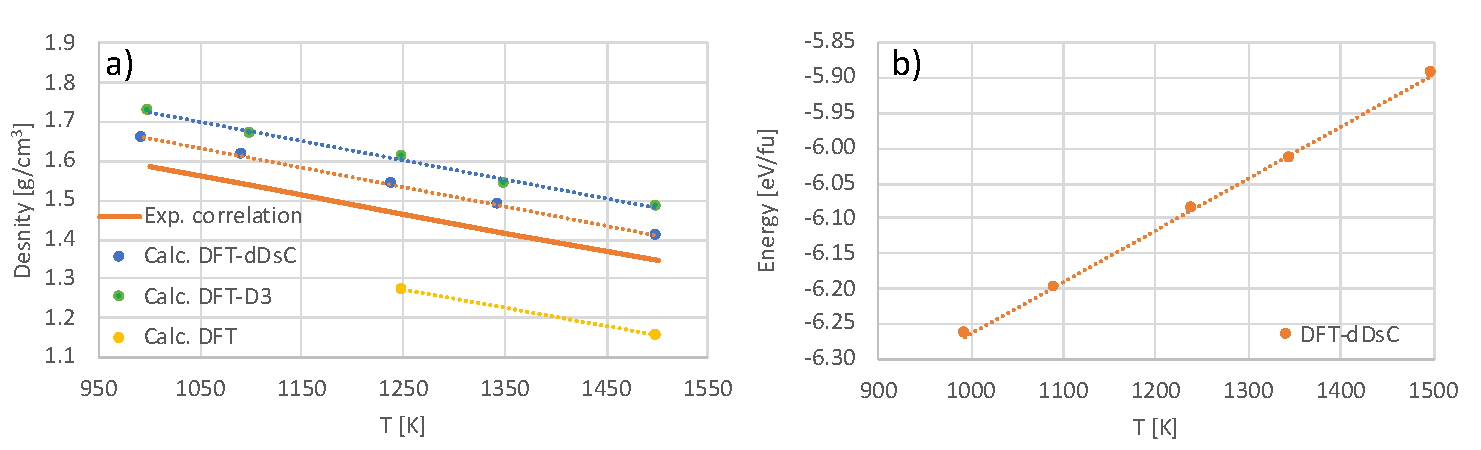
\includegraphics[width=0.95\textwidth]{FIG2.pdf}
\caption{a) Density of NaCl predicted with two different models for dispersion forces (D3 and dDsC) and one without (small cell for dDsC, large cell for others). Experimental data is represented by the correlation plotted as an orange line~\cite{Janz1988}. b) Calculated total energy of NaCl as function of temperature (small cell). The line is a least-squares fit to data points and the slope represents the heat capacity.} %Note that the temperature range of the experimental correlation and some data points extend beyond the boiling point of NaCl, which is solely for illustrative purposes. 
%The lines shown are least-squares fits to the calculated data points.} 
\label{fig:NaCldensity}
\end{figure}

%\begin{figure}[htb]
%\centering
%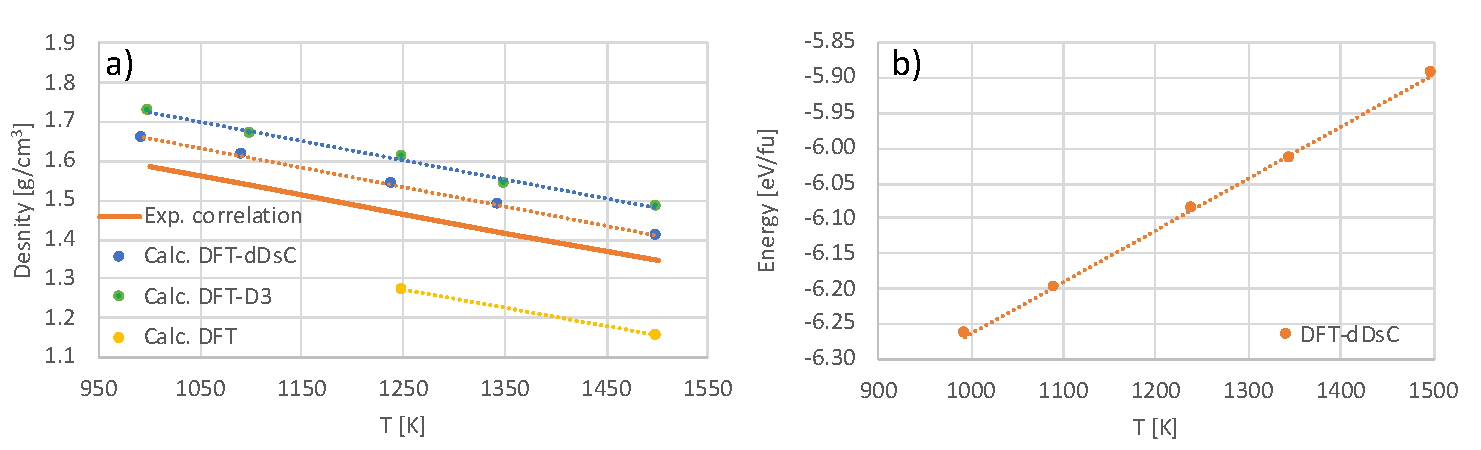
\includegraphics[width=0.45\textwidth]{FIG2.pdf}
%\caption{Density of NaCl predicted with three different models for dispersion forces and one without. Experimental data is represented by the correlation plotted as an orange line~\cite{}. %Note that the temperature range of the experimental correlation and some data points extend beyond the boiling point of NaCl, which is solely for illustrative purposes. 
%The lines shown are least-squares fits to the calculated data points.} 
%\label{fig:NaClpair}
%\end{figure}

\begin{table*}[hb!]
\centering
\begin{tabular}{lcc}
\hline
\hline
& Density (g/cm$^3$) &Heat capacity (J/mol/K) \\
%%&a &b &b \\
\hline
%NaCl Calculated (D3)	& &  \\
NaCl Calculated (dDsC)	&$2.1594-0.0004993T$ &71.6 \\
%%NaCl Calculated (Langreth \& Lundqvist)	& & & & & & \\
NaCl Experiment	&$2.061-0.0004759T$~\cite{Janz1988} &66.9~\cite{NIST}  \\
%UCl$_3$ Calculated (Langreth \& Lundqvist) & & & & & & \\	
UCl$_3$ Calculated (dDsC) &$6.1066-0.001383T$ &145.3 \\	
UCl$_3$ Experiment	&$6.375-0.001522T$~\cite{Desyatnik} &150~\cite{McMurray} \\
\hline
\hline
\end{tabular}
\caption{Calculated and experimental correlations and values for density and heat capacity of NaCl and UCl$_3$.}% The first quantity is a linear function of temperature, while the latter two are constants.}
\label{table:NaCldensityetc}
\end{table*}

\subsubsection{Heat capacity} 
Figure \ref{fig:NaCldensity}b plots the total energy per formula unit of molten NaCl as function of temperature. The derivative equals the heat capacity of NaCl, which is also tabulated in Table \ref{table:NaCldensityetc} together with an experimental reference value~\cite{NIST}. The results refer to the supercell size that we consider best converged for each methodology, see caption and below for further discussion. The simulation results indicate a constant heat capacity, though in order to identify small deviations from this behavior a denser temperature mesh would be required. The good agreement between simulations and experiments for the heat capacity (see Table \ref{table:NaCldensityetc}) further emphasizes the accuracy of the AIMD simulations. 

%\begin{figure}[htb]
%\centering
%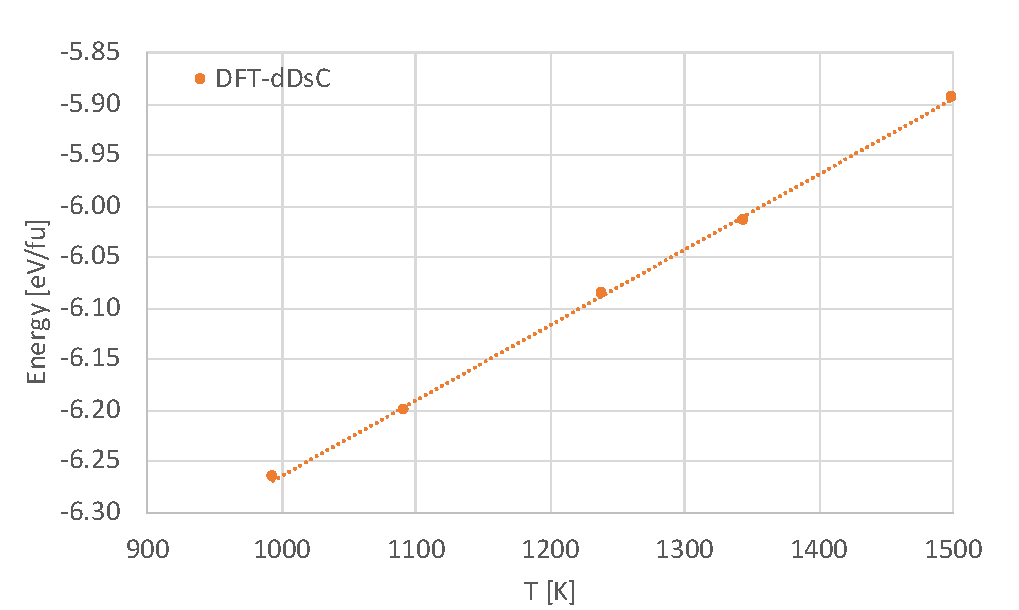
\includegraphics[width=0.95\textwidth]{FIG3.pdf}
%\caption{Calculated total energy of NaCl as function of temperature (small cell). The line is a least-squares fit to data points and the slope represents the heat capacity.} 
%\label{fig:NaClheatc}
%\end{figure}

\subsubsection{Impact of supercell size and other simulation settings}
The results in Figure \ref{fig:NaCldensity} refer to simulations based on the supercell that we consider best converged. Figure \ref{fig:NaClsize} compares these results with those obtained from other supercells. Density and heat capacity are accurately represented by all supercell sizes in the temperature range investigated.
%smaller supercells, at least below 1750 K, which supports the accuracy of the results with respect to the supercell size. 
 These results suggest that for NaCl, the larger supercell is not required to achieve converged results for density and heat capacity at moderate temperature, which is consistent with the discussion of radial distribution functions in Sec. \ref{sec:method}. The small variations between supercells are more likely related to sampling differences, rather than due to the supercell size. Consequently, the converged results in Figure \ref{fig:NaCldensity} as well as the correlations in Table \ref{table:NaCldensityetc} are representative of all simulation results in this study, regardless of the supercell size. %Some deviation is observed for the highest temperature, which may be related to approaching the boiling temperature. 

\begin{figure}[htb]
\centering
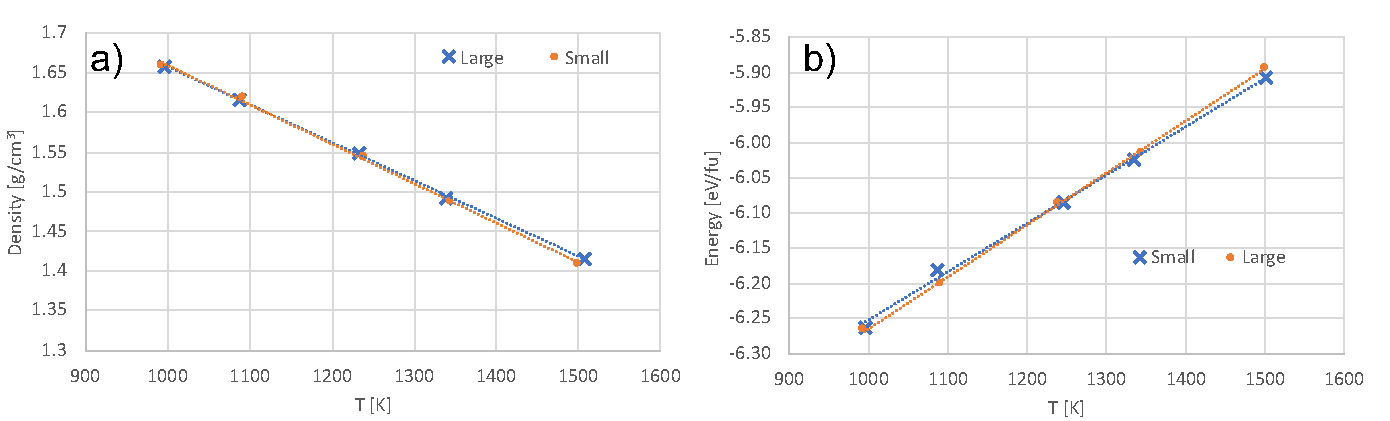
\includegraphics[width=1.00\textwidth]{FIG3b.pdf}
\caption{a) Calculated density and b) total energy of NaCl as function of temperature for the large and small supercells. The lines are least-squares fits to data points and the slope represents the heat capacity.} 
\label{fig:NaClsize}
\end{figure}

%The NVT simulations also allow calculation of the compressibility and diffusivity of each species. These results are also summarized in Table \ref{table:NaCldensityetc} (compressibility) and Table \ref{table:NaCldiffusivityetc}.

\subsection{Ab initio molecular dynamics simulations on UCl$_3$}
\subsubsection{Density and structure}
Following the results for NaCl, the best performing Van der Waals model (dDsC) was applied to UCl$_3$. % with a few spot checks using the other Van der Waals models as well. 
Figure \ref{fig:UCl3density}a) plots the predicted density for UCl$_3$ as function of temperature for the dDsC dispersion model. 
These results refer to the supercell size that we deem to be best converged and most representative of the UCl$_3$ system, see below for further discussion. 
The figure also compares the predicted densities to two literature correlations derived from experiments~\cite{Janz1988,Desyatnik}.
%The inset highlights the difference in energy between the AFM, FM and non-magnetic simulations. 
%Figure \ref{fig:UCl3density}b) also includes results from simulations that do not include the Hubbard $U$ model for the U 5f electrons. 
The two experimental correlations for density are surprisingly different and cannot both be correct, except in a narrow temperature range. 
% The most recent experimental data set agrees well with the simulation data, with both the Langreth \& Lundqvist and dDsC model predicting values within a few per cent of the experimental data. 
 The temperature dependence is predicted to be close to linear across the full temperature range investigated and agrees very well with the experimental data due to Desyatnik et al.~\cite{Desyatnik}. %The Langreth \& Lundqvist methodology is sensitive to the choice of exchange -correlation potential. The optimal choice proved excellent agreement with experiments, while other choices may lead to significant underestimation of the density despite performing very well for the NaCl benchmark system. 
 %Note that only a single point was calculated for the DFT-D3 model, but that indicates essentially the same behavior as the dDsC model.  
 %Compared to the Desytniak et al. correlation~\cite{Desyatnik}, the predicted temperature dependence of the density is slightly different. 
 The densities in Figure \ref{fig:UCl3density} were fitted to linear correlations and summarized in Table \ref{table:NaCldensityetc}. 
 
The radial pair distribution function at 1250 K is reported in Figure \ref{fig:radial}, which highlights a first-shell coordination distance of 2.82~\AA. The coordination distance is in excellent agreement with the experimental values of 2.82 \AA~\cite{Neilson} and 2.84 \AA~\cite{Okamoto} measured at 1113 K and 1200 K, respectively, while it is higher than the AIMD simulations by Li et al.~\cite{Li}, which can likely be ascribed to the application of the Hubbard $U$ methodology in the present study. The predicted coordination numbers are within the 6 to 8 range reported in experiments and previous simulations~\cite{Li,Neilson,Okamoto}. %The U-U radial distribution function tends to zero slower than the 
 
% The effect of including the Hubbard $U$ model is to decrease the density (increase the volume) compared to the reference case, which is consistent with the increase in volume observed for solid state simulations using the Hubbard $U$ methodology. The results without the Hubbard $U$ parameter is slightly closer to the densities measured in experiments. The magnetic order has a very small influence on the predicted density, which is highlighted in Figure \ref{fig:UCl3density}b). %We believe that the AFM (random) distribution is more representative of the high-temperature behavior of molten salts, as it should exhibit the lowest free energy (see below).

\begin{figure}[htb]
\centering
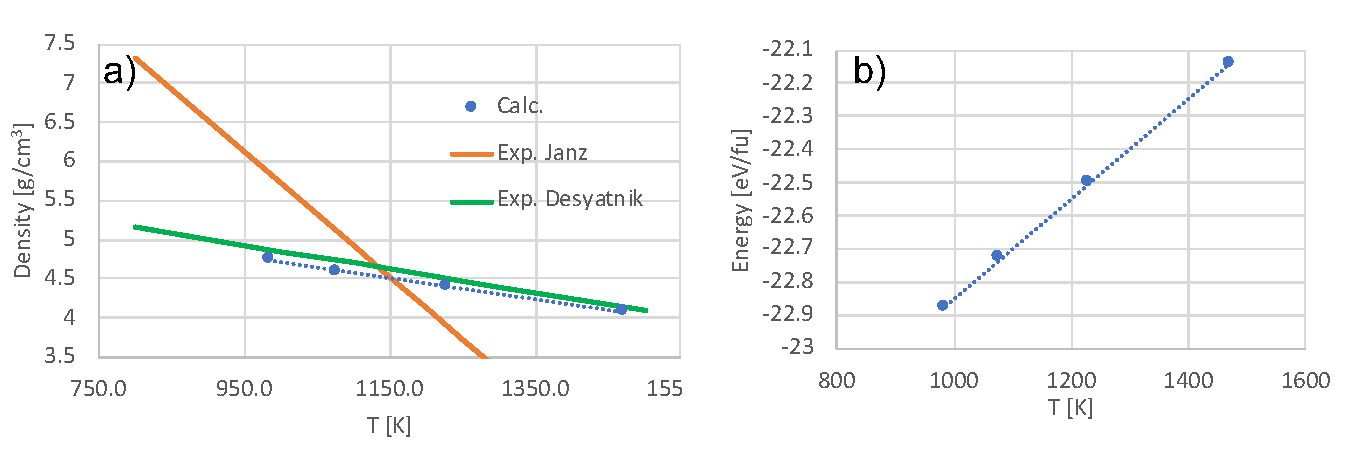
\includegraphics[width=1.00\textwidth]{FIG4.pdf}
\caption{a) Density of UCl$_3$ predicted the dDsC model for the dispersion forces (small cell). Experimental data is represented by the correlations plotted as green~\cite{Desyatnik} and orange lines~\cite{Janz1988}. The dashed line is a least-squares fit to the calculated data points, the equations of which are summarized in Table \ref{table:NaCldensityetc}. b) Calculated total energy of UCl$_3$ as function of temperature (small cell). The line is a least-squares fit to data points and the slope represents the heat capacity.} 
\label{fig:UCl3density}
\end{figure}

\subsubsection{Heat capacity} 
Figure \ref{fig:UCl3density} plots the total energy as function of temperature, from which the heat capacity can be derived by calculating the slope. The total energy closely follows a linear relation as function of temperature and, consequently, the heat capacity can be approximated as a constant in the temperature range investigated. In order to resolve small deviations from the linear relation, a denser temperature mesh would have to be used. 
Experimental data for the heat capacity of UCl$_3$ has not been identified, but our results compare very well with the value derived from the MSTDB CALPHAD assessment of the UCl$_3$ thermodynamics (see Table~\ref{table:NaCldensityetc})~\cite{McMurray}. %Figure \ref{fig:fig:UCl3heat}b compares the total energy as function of temperature for simulations assuming different magnetic ordering. The AFM (random) ordering is predicted to be slightly more stable than the FM ordering, though the difference is small. The AFM (random) model would be further stabilized by the magnetic entropy originating from the random distribution of magnetic moments at finite temperature. Consequently, the AFM (random) distribution of magnetic moments is considered to be the most representative model. %, which confirms AFM (random) ordering as the most appropriate model for production simulations. 

%\begin{figure}[htb]
%\centering
%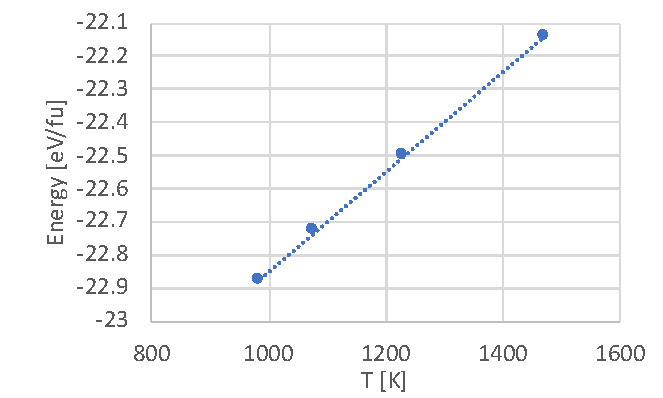
\includegraphics[width=0.95\textwidth]{FIG5.pdf}
%\caption{Calculated total energy of UCl$_3$ as function of temperature (small cell). The line is a least-squares fit to data points and the slope represents the heat capacity.} 
%\label{fig:UCl3heat}
%\end{figure}

%\subsubsection{Diffusivity}
%As for NaCl, The AIMD simulations also allow calculation of the diffusivity of each species. Again similar to the NaCl system, these simulations work best in the NVT ensemble and results are only report for that case, see Fig. \ref{fig:diffUCl}. As expected, the diffusivity is a linear function of temperature. %, with a much stronger temperature dependence for Cl than for U. 
%The mobility of each species may be derived from the slope of the diffusivity as function of temperature (see Table \ref{table:NaCldiffusivityetc}). 

%\begin{figure}[htb]
%\centering
%\includegraphics[width=0.45\textwidth]{FIGDiffUCl.pdf}
%\caption{Calculated diffusivities for each species in NaCl as function of temperature.} 
%\label{fig:diffNaCl}
%\end{figure}

\subsubsection{Impact of supercell size and other simulation settings}
The results discussed above for UCl$_3$ refer to simulations using the supercell size that we deem to be best converged and most representative of the UCl$_3$ system for each simulation methodology. Select results obtained from different supercell sizes are compared in Figure \ref{fig:UCl3size}, which exhibits fairly good agreement with each other.  Any difference between supercell sizes is primarily ascribed to sampling appropriate configurations rather than an effect of increasing the numbers of ions in the simulation box, although additional simulations would be required to fully certify this conclusion. Compared to NaCl it is much more challenging to reach long simulation times for the large UCl$_3$ simulation cells. 

\begin{figure}[htb]
\centering
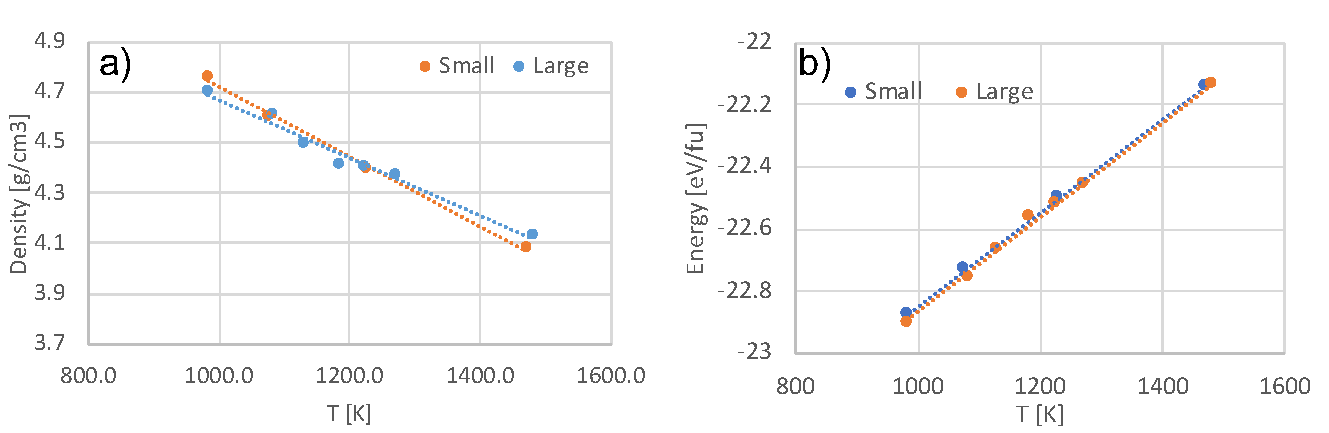
\includegraphics[width=1.00\textwidth]{FIG4b.pdf}
\caption{Calculated density and total energy of UCl$_3$ as function of temperature for the large and small supercells. The line is a least-squares fit to data points and the slope represents the heat capacity.} 
\label{fig:UCl3size}
\end{figure}

%As for NaCl, The NVT simulations also allow calculation of the compressibility and diffusivity of each species. These results are  summarized in Table \ref{table:NaCldensityetc} (compressibility) and Table \ref{table:NaCldiffusivityetc}.
 
\subsection{Ab initio molecular dynamics simulations on NaCl-UCl$_3$}
\subsubsection{Density and structure}
The density of NaCl-UCl$_3$ mixtures were calculated for the dDsC dispersion model at three or four (depending on composition) different temperatures between 800 K and 1500 K, as shown in Figure \ref{fig:NaClUCl3}a). This figure also includes densities at the same temperatures as those of the simulations obtained from correlations derived from experimental data due to Desyatnik et al.~\cite{Desyatnik}. %and lines corresponding to an ideal mixture of the end members. 
Figure \ref{fig:NaClUCl3}b) highlights the fractional deviation from ideal solution behavior as calculated from simulations and experiments~\cite{Desyatnik}. 
It is challenging to converge the density for mixed salt solutions to an accuracy better than around one per cent of the absolute density using AIMD simulations, which gives rise to some scatter in the data points. 
Nevertheless, a few trends are discernible from Figure \ref{fig:NaClUCl3}. The simulated data points are within a few per cent of the experimental data.  %and close to an ideal mixture. 
The simulations suggest a negative deviation from an ideal solution (lower density than predicted by an ideal solution behavior) by up to 2-3\%, except close to pure UCl$_3$ at high temperature where a positive deviation is observed. According to our simulations, the magnitude of the deviation from ideal solution behavior is a function of composition and varies some with temperature starting at $x_{UCl_3}\approx0.35$ and continuing in the UCl$_3$ rich composition range, while it is almost independent of temperature in the NaCl rich range. 
The maximum deviation from ideal solution behavior occurs close to the eutectic composition of 35\% UCl$_3$. These predictions are qualitatively similar to the correlations derived form experiments by Desyatnik et al.~\cite{Desyatnik}, though the experimental correlations predict a larger magnitude for the deviation from an ideal solution and also exhibit a stronger temperature dependence than the simulations. %The Langreth \& Lundqvist simulations within the NVT ensemble predict a close to ideal solution behavior across the full temperature and composition range.
  %  and experiments suggest a negative deviation from an ideal solution (lower density than predicted by an ideal solution behavior), except close to pure UCl$_3$ where experiments and simulations at T=1500K exhibit a positive deviation. Although experiments report the magntiude of the deviation from ideal solution to be a function of temperature, the highest deviation occurs at low temperatures, simulations predict a close to temperature independent deviation from ideal solution behavior. Both experiments and simulations predict a minimum in the deviation rom ideal solution close to the eutectic composition of 30\%, however simulations predict the magnitude of the deviation to be much smaller than experiments. 
%It is challenging to converge the density for mixed salt solutions using AIMD simulations, which give rise to some of the 
% . Although there is some spread in the data points that we ascribe to sampling uncertainties, there is a minimum about 3\% below the ideal solution density close to the eutectic composition. The experimental data also shows a negative deviation, including a minumum close to the eutectic composition.  

Figure \ref{fig:NaClUCl3_t}a) plots the density as function of temperature for each composition, which emphasizes a close to linear temperature dependence, similar to the pure end-members. %The corresponding linear equations for each composition are listed in Table \ref{table:density_data}. 
The coefficients describing the linear dependence on temperature for each composition are plotted in Figure \ref{fig:NaClUCl3_comp}a). Although there is some scatter, a weak non-linear dependence on composition for both the linear and constant term (not shown) is identified. The non-linear dependence is most pronounced in the UCl$_3$ rich range.  
%except for $x_{UCl_3}=0.875$, which deviates slightly from the general trend for both parameters. %The weak non-linear composition dependence can be parametrized and used to express the temperature and composition dependent densities according to:
%\begin{equation}
%\end{equation}
The density correlations identified in Figures \ref{fig:NaClUCl3_t}a) and \ref{fig:NaClUCl3_comp}a) can, in principle, be used for calculating densities at temperatures and compositions not explicitly investigated by AIMD simulations. % according to the following equations,
%This approach is utilized to compare the AIMD predictions to the recent experimental data from Scott et al.~\cite{} in Fig. \ref{fig:NaClUCl3_comp} collected at XX and YY K. These experiments suggest that the density behaves much closer to an ideal solution than those due to Desyatnik et al.~\cite{}. The agreement with the AIMD predictions is still very good, considering uncertainties associated with both experiments and simulations.  

\begin{figure}[htb]
\centering
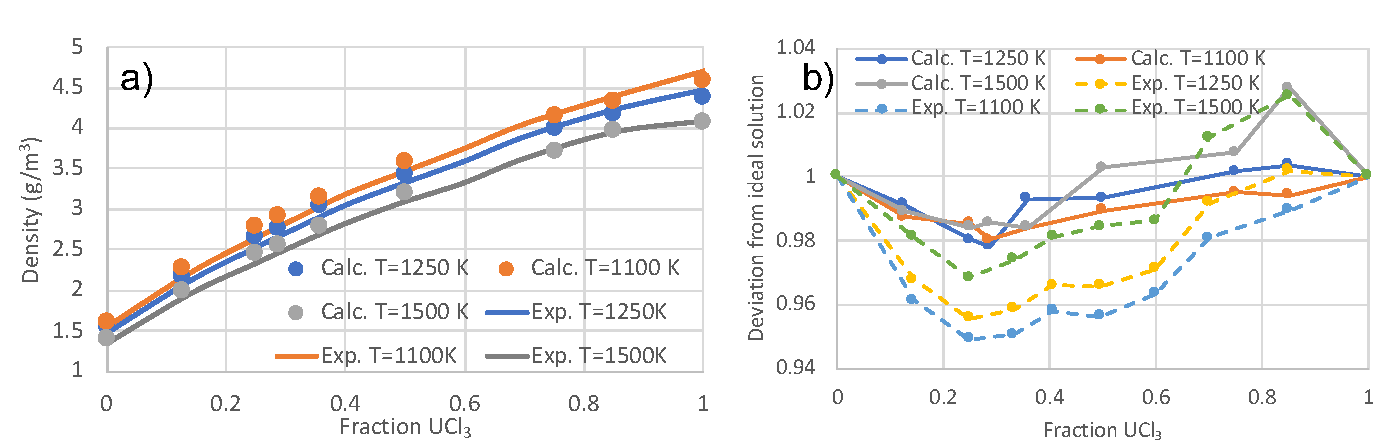
\includegraphics[width=1.00\textwidth]{FIG6.pdf}
\caption{a) Density of NaCl-UCl$_3$ mixtures as obtained from simulations and experimental data~\cite{Desyatnik} at temperatures between 1100 K and 1500 K. %The lines represent an ideal solution with the calculated and experimental NaCl and UCl$_3$ densities as end points. 
b) The fractional deviation form ideal solution behavior plotted as function of composition at temperatures between 1100 K and 1500 K. %Results for both the large and small supercells are shown.
} 
\label{fig:NaClUCl3}
\end{figure}

\begin{figure}[htb]
\centering
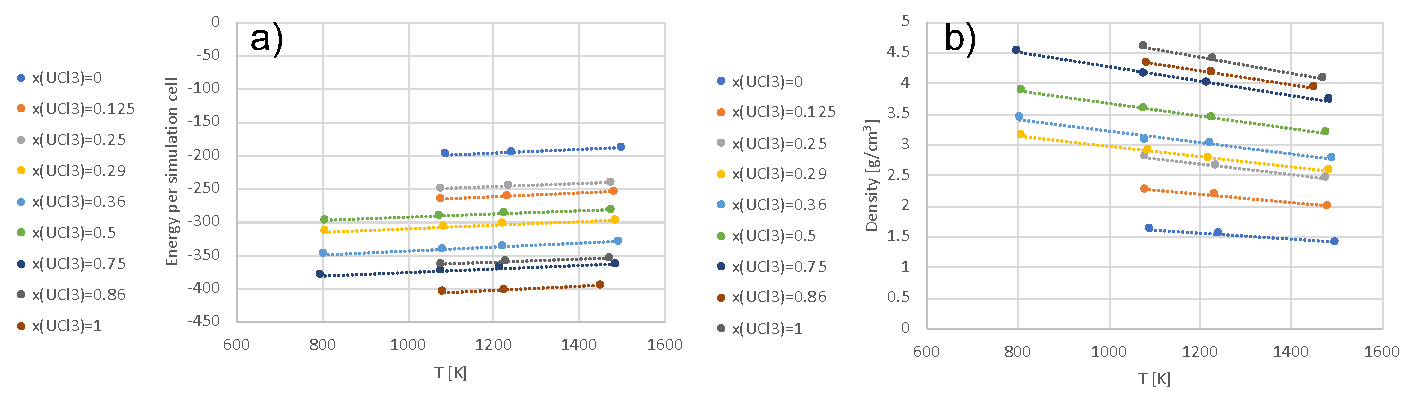
\includegraphics[width=1.00\textwidth]{FIG6c.pdf}
\caption{a) Calculated temperature dependent densities as function of composition. b) Calculated energies per simulations cell as function of composition. In both a) and b) the lines represent least-squares fits to the calculated data.}  
\label{fig:NaClUCl3_t}
\end{figure}

\begin{figure}[htb]
\centering
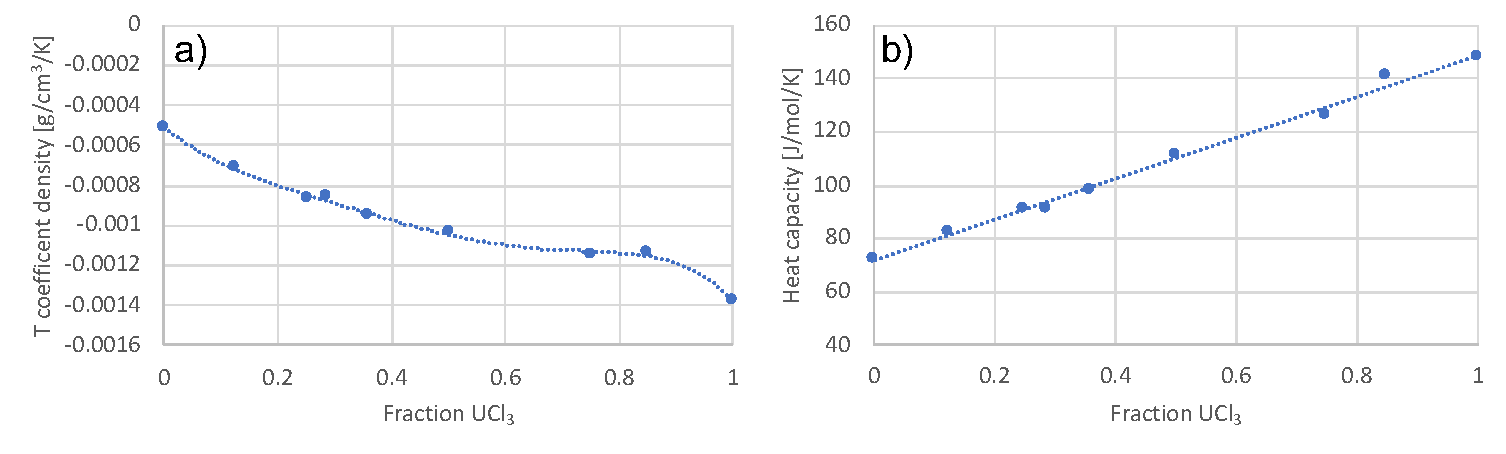
\includegraphics[width=1.00\textwidth]{FIG6f.pdf}
\caption{a) Coefficient describing the linear temperature dependence of density as function of the UCl$_3$ fraction. The line represents a least-squares fit of a fifth order polynomial. b) Heat capacity as function of the UCl$_3$ fraction. The line represents a least-squares fit of a linear correlation.}
\label{fig:NaClUCl3_comp}
\end{figure}

\subsubsection{Mixing energy and heat capacity}
The mixing energies of NaCl-UCl$_3$ at temperatures ranging from 1100 K to 1500 K are plotted in Figure \ref{fig:NaClUCl3e}a), with the NaCl and UCl$_3$ end members as reference points. The mixtures exhibit a negative deviation from ideal solution behavior, which implies that the solution phase is favored over a two-phase mixture of the end-points. Addition of entropy further stabilizes the mixed solution phase, as shown in Figure \ref{fig:NaClUCl3e}b) by adding a simple ideal solution model to the potential energy in Figure \ref{fig:NaClUCl3e}a).
 The minimum (most negative) mixing energy is between $x_{UCl_3}$=0.35 and  $x_{UCl_3}$=0.5, which qualitatively mimics the results for the density. %The potential energy minimum may be shifted slightly closer to the 50-50 composition. However, it may be questionable if the simulations are sufficiently converged to draw such a subtle conclusion.  The Langreth \& Lundqvist and dDsC simulations predict very similar solution energies. The minimum of the free energy is shifted close to the 50-50 composition. 
 
 The mixing energy was measured at 1100 K by Matsuura et al.~\cite{Matsuura} The results are also shown in \ref{fig:NaClUCl3e}a) and indicate very good agreement with the simulations across the full temperature range. In addition to the experimental data points, there are two sets of thermodynamic models for the solution energy~\cite{BENES2008,YIN2020}, see Figure \ref{fig:NaClUCl3e}a) for the correlation from Ref.~\cite{YIN2020}. Both thermodynamic models assume the solution energy to be independent of temperature, which is in good agreement with the simulations. The model by Yin et al.~\cite{YIN2020} was derived from the experimental measurements by Matsuura et al.~\cite{Matsuura} and consequently agree similarly well with our simulation results. The model by Benes et al.~\cite{BENES2008} exhibits a smaller mixing energy than both the experimental data points and our simulations (not shown). 

%Although the simulations were run long enough to sample the configuration space, it is possible that the initial distribution of Na and U ions have some impact on the results, especially for the large supercells.  In order to test this possibility, a few of the Na And Cl atoms in the previous simulations were swapped and the simulations were re-run. In particular we target the compositions that seemed to deviate from the overall trend somewhat. Indeed, the new simulations provided slightly different results in closer agreement with the trends already discussed. For the large cells, this is an inherent uncertainty of the simulation apporach.

\begin{figure}[htb]
\centering
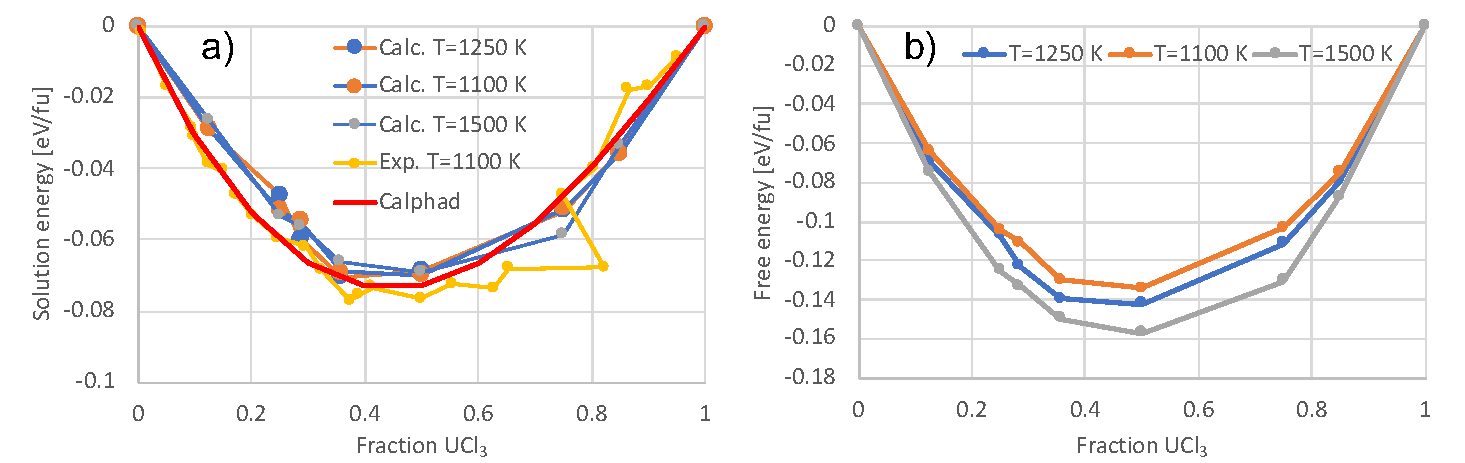
\includegraphics[width=1.00\textwidth]{FIG7.pdf}
\caption{a) Mixing energies for NaCl-UCl$_3$ at 1100, 1250 and 1500 K. Pure NaCl and UCl$_3$ are used as references. The calculated results are compared to experiments~\cite{Matsuura} and a thermodynamic assessment~\cite{YIN2020}.%The solid black line represents the zero-mixing energy for the ideal solution. %b) Same as a) but performed using a different simulation methodology at 1200 K. 
 Results are shown for the best converged supercells. b) The free energy of mixing at 1100 1250 and 1500 K assuming an ideal solution.} 
\label{fig:NaClUCl3e}
\end{figure}

The total energy for each NaCl-UCl$_3$ composition is plotted as function of temperature in Figure \ref{fig:NaClUCl3_t}b), from which heat capacity can be calculated as the slope, similar to the pure NaCl and UCl$_3$ systems. The heat capacity is a linear function of the salt composition, which is expected based on the lack of temperature dependence for the salt mixing energies. The negative deviation from an ideal solution seen for the mixing energy and density is not present for the heat capacity. 

%Based on the results for the mixing energy and heat capacity, the following expression may be derived for the mixing energy as function of the composition and temperature:
%\begin{equation}
%\end{equation}

%The comparison between large and small supercells for the density and mixing energy are also shown in Figs. \ref{fig:NaClUCl3} and \ref{fig:NaClUCl3e}. Unlike the cases of NaCl and UCl$_3$, the NaCl-UCl$_3$ mixture exhibit some deviation between the supercells for one of the compositions, although the trends are still the same. 

\section{Discussion}
\label{sec:discussion}
This discussion section will focus on the behavior of mixed salts, in particular how the mixing properties (energy and density) relate to the evolution of the pair distribution functions in the mixed salts. Figure \ref{fig:fig_pair} plots the pair distribution functions at four salt compositions ($x_{UCl_3}=0.25$, $x_{UCl_3}=0.29$, $x_{UCl_3}=0.36$ and $x_{UCl_3}=0.50$) and compares them to the reference pair distribution functions for UCl$_3$. 
Ref.~\cite{Li} already showed that as NaCl is added to pure UCl$_3$, the number of Cl ions in the first neighbor shell around U ions increases, from 6 in UCl$_3$ to almost 8 close to NaCl, with a corresponding decrease around Na ions. This is also confirmed in the present study (see the increase of the first peak in Figure \ref{fig:fig_pair} as the NaCl fraction increases). This redistribution of Cl ions clearly represents a favorable interaction as the mixing energy is negative across the full composition range. The same study also identified networks of UCl$_3$ units above a fractional UCl$_3$ concentration of 0.30, and more isolated units below this concentration. This behavior is also visible in the pair distribution functions. The U-U pair distribution function for mixtures with a composition equal to or above a fractional UCl$_3$ concentration of 0.36 maintain the same shape and height as in pure UCl$_3$ (they essentially overlap), which emphasizes the importance of network formation in the mixtures. 
Below a fractional concentration of 0.36 the U-U pair distribution function rapidly deviates from the pure UCl$_3$, indicating an inability to maintain the favorable network structure. This behavior is visible in the third coordination shell in Figure \ref{fig:fig_pair}.
Related changes may be observed in other distribution functions. 
The location of this transition coincides with the minimum in the mixing energy and the maximum deviation of the density from an ideal solution (compare Figures \ref{fig:fig_pair}, \ref{fig:NaClUCl3} and \ref{fig:NaClUCl3e}). In turn, these coincide with the eutectic composition according to the experimental phase diagram~\cite{YIN2020}. Combined with the evolution of the U-Cl and U-U pair distribution functions in the mixtures, this suggests that the negative mixing energy is driven by increases in the Cl coordination around U ions, but if the fractional UCl$_3$ concentration is below $\approx 0.36$, the gain from increasing this U-Cl coordination is countered by not being able to maintain the favorable U-U coordination seen in UCl$_3$, as evidenced by the break-up of the network structure. The balance of the increase in the U-Cl coordination and decrease in U-U coordination as function of the composition of NaCl-UCl$_3$ salts is responsible for the minimum in the mixing energy and by extension the location of the eutectic point in the phase diagram. 

The negative deviation from an ideal solution exhibited by the density implies that the volume increases. Often, a negative mixing energy is associated with a stronger bonding and lower volume, clearly that is opposite to what is observed for NaCl-UCl$_3$. The reason for increased volume and decreased density is again related to the evolution of the pair distribution function. The increased coordination number of Cl around U ions means that the bonding environment starts to resemble that of U$^{4+}$ ions in UCl$_4$, which may also be what drives the favorable interaction. The density of UCl$_4$ is noticeably lower (and the molar volume higher) than that of UCl$_3$, which we believe correlates with the negative deviation form an ideal mixture for the density of NaCl-UCl$_3$ mixtures. Note that this analogy does not imply  presence of formal U$^4+$ ions in NaCl-UCl$_3$, but a partial transition that drives the evolution of both the mixing energy and density. Additional simulations and experiments would be required to prove this hypothesis.

 \begin{figure}[htb]
\centering
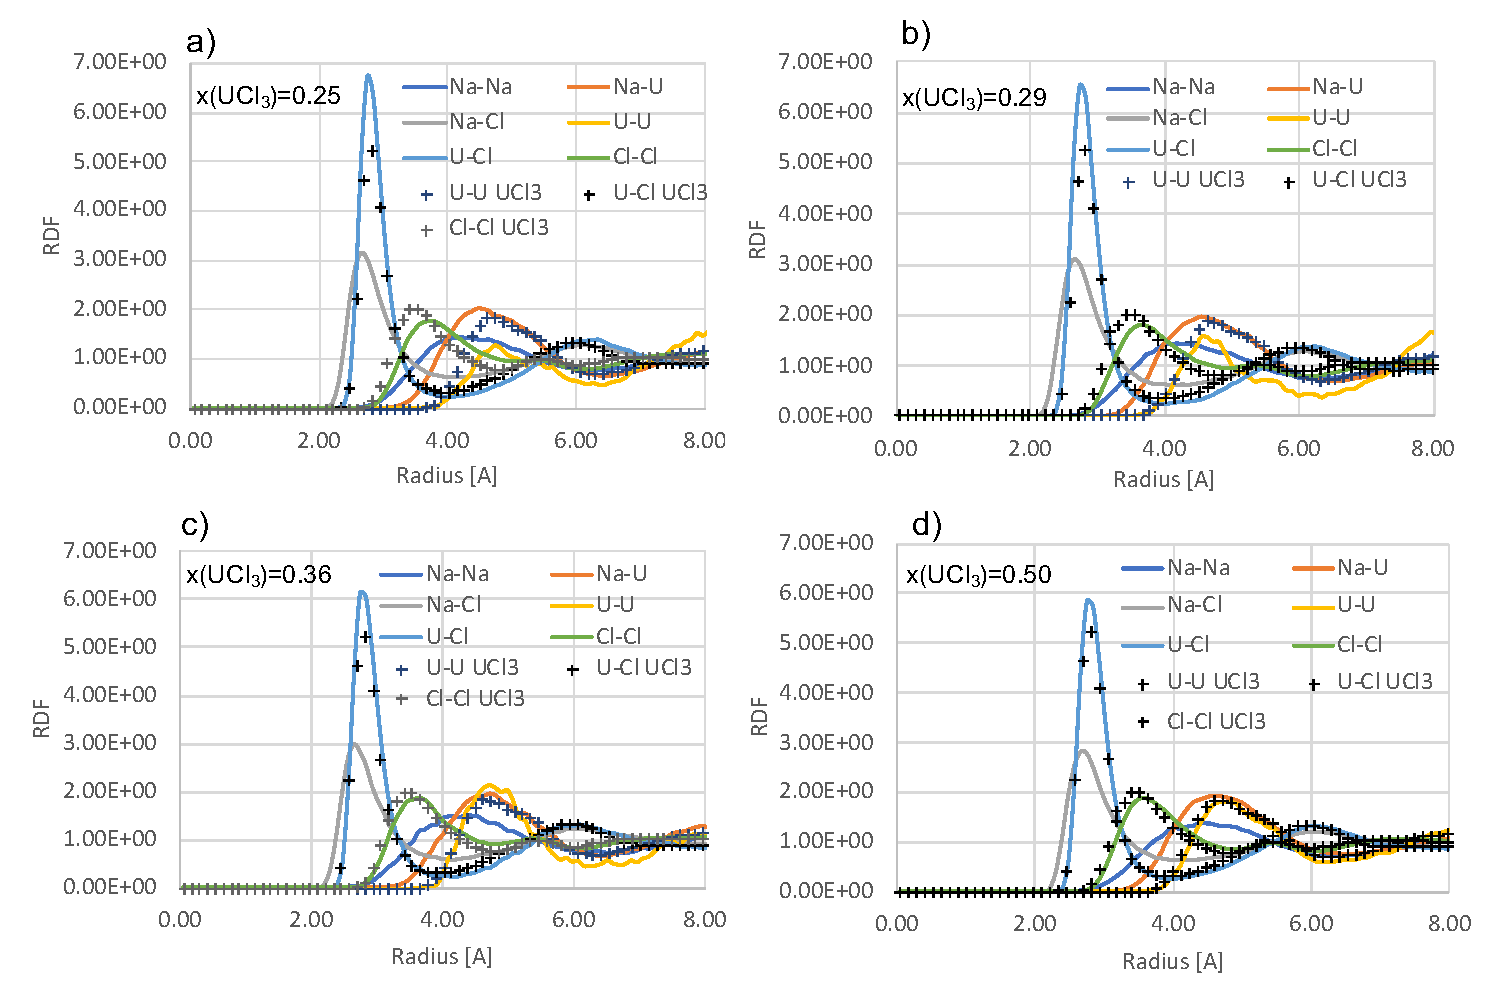
\includegraphics[width=1.00\textwidth]{FIG77.pdf}
\caption{Pair distribution functions for NaCl-UCl$_3$ mixtures as function of composition ($x_{UCl_3}=0.25$, $x_{UCl_3}=0.29$, $x_{UCl_3}=0.36$ and $x_{UCl_3}=0.50$). The reference U-Cl and U-U pair distribution functions for UCl$_3$ are plotted in each figure for comparison.} 
\label{fig:fig_pair}
\end{figure}

\chapter{Summary and conclusions}

\bibliographystyle{elsarticle-num}         
\bibliography{Yellowjacket.bib}

\end{document}
